%%%%%%%%%%%%%%%%%%%%%%%%%%%%%%%%%%%%%%%%%
% Original author:
% Linux and Unix Users Group at Virginia Tech Wiki
% (https://vtluug.org/wiki/Example_LaTeX_chem_lab_report)
% Modified by: Hector F. Jimenez S, for the Digital Electronics Laboratory.
% License:
% CC BY-NC-SA 3.0 
%%%%%%%%%%%%%%%%%%%%%%%%%%%%%%%%%%%%%%%%%
%----------------------------------------
%	PACKAGES AND DOCUMENT CONFIGURATIONS
%---------------------------------------
\documentclass[paper=a4, fontsize=12pt]{article} 		% A4 paper and 11pt font size
\usepackage[T1]{fontenc} 								% Use 8-bit encoding that has 256 glyphs
%\usepackage{fourier}		 							% Use the Adobe Utopia font for the document 
\usepackage[spanish,english]{babel}						% Spanish Language, templates uses some sections in english.
\selectlanguage{spanish}								% main language.
\usepackage{subfig}
\usepackage{multirow}
\PassOptionsToPackage{spanish}{babel}
\renewcommand{\figurename}{Figura}						% Force rename of figure.
\renewcommand{\figurename}{Fig.}
\usepackage[figurename=Fig.]{caption}
\usepackage[utf8]{inputenc}								% tildes for spanish language.
\usepackage{amsmath,amsfonts,amsthm} 					% Math packages.
\usepackage{minted}										% For syntax highlighting.
	    \renewcommand\listingscaption{Código}			%rename the source code minted !
\usepackage{float}										% Image will be in the same place as you want.!!! x-/
\usepackage{sectsty} 									% Allows customizing section commands
\allsectionsfont{\centering \normalfont\scshape}	   	% Make all sections centered, the default font and small caps
\usepackage{hyperref}
\hypersetup{											%Setups the false color and borders.
    colorlinks=false,
    pdfborder={0 0 0},
}
\newcommand\fnurl[2]{%									% set a simple and quick footnote command and include url.
\href{#2}{#1}\footnote{\url{#2}}%	
}
\usepackage{graphicx}									% Import easyly images.
\graphicspath{ {./images/} }							% Where to look for the images.
\DeclareGraphicsExtensions{.pdf,.png,.jpg}				% Graphics Extension to be used
\usepackage[notes,backend=biber]{biblatex-chicago}		% Bibliography and references.
\bibliography{biblio}									% bibliography filename.
\usepackage{fancyhdr} 									% Custom headers and footers
\pagestyle{fancyplain} 									% Makes all pages in the document conform to the custom headers and footers
\fancyhead{} 											% No page header
\fancyfoot[L]{} 										% Empty left footer
\fancyfoot[C]{} 										% Empty center footer
\fancyfoot[R]{\thepage} 								% Page numbering for right footer
\renewcommand{\headrulewidth}{0pt} 						% Remove header underlines
\renewcommand{\footrulewidth}{0pt} 						% Remove footer underlines
\setlength{\headheight}{13.6pt} 					    % Customize the height of the header
\numberwithin{equation}{section}						% Number equations within sections (i.e. 1.1, 1.2, 2.1, 2.2 instead of 1, 2, 3, 4)
%\numberwithin{figure}{section} 						% Number figures within sections (i.e. 1.1, 1.2, 2.1, 2.2 instead of 1, 2)
\numberwithin{table}{section} 							% Number tables within sections (i.e. 1.1, 1.2, 2.1, 2.2 instead of 1, 2, 3, 4)
\setlength\parindent{0pt} 								% Removes all indentation from paragraphs
\newcommand{\horrule}[1]{\rule{\linewidth}{#1}} 		% Create horizontal rule command with 1 argument of height
\usepackage{listings}% http://ctan.org/pkg/listings
\usepackage{multicol}
\usepackage{caption}
\usepackage{subfig}
\renewcommand{\lstlistingname}{Código}	
\title{Sistemas Operativos I\\ 
\horrule{0.5pt} \\[0.4cm] 								% Thin top horizontal rule	Title rule
\textit{Taller 6: Caso de estudio del sistema operativo Solaris 10}
\horrule{1pt} \\[0.5cm] 			
} 			

\author{												
Héctor F. \textsc{Jiménez Saldarriaga.}\\				% Authors begin.
\texttt{hfjimenez@utp.edu.co} \\						
\texttt{PGP KEY ID: 0xB05AD7B8}
} 
% End of  Author name
\date{}    						                       % Date for the report, this will hide the \today.

\begin{document}
\maketitle                      			           % Insert the title, author and date
\begin{center}
\begin{tabular}{l r}								   % two column to
Fecha de Entrega: & Marzo, 2018 \\				   % Ramiro's Details.
Profesor: & Cesar Manuel Castillo Rodriguez
\end{tabular}
\end{center}
%%%%%%%%%%%	
% Let's start the document.
%%%%%%%%%%%	
\section{Objetivos}
\begin{itemize}
	\item Evolución
	\item Realizar el proceso de instalación del sistema operativo	
    \item Identificar el manejo de Archivos, Shell
    \item Estructura del Sistema Operativo
    \item Clasificación del Sistema Operativo
	\item Ejecución de Comandos, al menos 20.
\end{itemize}
\section{Historia y Evolución de Solaris} 
La historia de este sistema operativo se encuentra adaptada  del sitio  web de wikipedia donde se describe una descripcion de lo que es Solaris:
\textit{ El primer sistema operativo de Sun nació en \textbf{1983} y se llamó inicialmente SunOS. Estaba basado en el sistema UNIX BSD, de la Universidad de California en Berkeley, del cual uno de los fundadores de la compañía fue programador en sus tiempos universitarios. Más adelante incorporó funcionalidades del System V, convirtiéndose prácticamente en un sistema operativo totalmente basado en System V. Esta versión basada en System V fue publicada en 1992 y fue la primera en llamarse Solaris, más concretamente \textbf{Solaris 2}. Las anteriores fueron llamadas Solaris 1 con efecto retroactivo. SunOS solo tendría sentido a partir de ese momento como núcleo de este nuevo entorno operativo Solaris. De esta forma Solaris 2 contenía SunOS 5.0. Desde ese momento se distingue entre el núcleo del sistema operativo (SunOS), y el entorno operativo en general (Solaris), añadiéndole otros paquetes como Apache o DTrace. Como ejemplo de esta función, Solaris 8 contiene SunOS 5.8.}

Solaris tiene una reputación de ser muy adecuado para el multiprocesamiento simétrico (SMP), soportando un gran número de CPUs. También ha incluido soporte para aplicaciones de 64 bits SPARC desde Solaris 7. Históricamente Solaris ha estado firmemente integrado con la plataforma hardware de Sun, SPARC, con la cual fue diseñado y promocionado como un paquete combinado. Esto proporcionaba frecuentemente unos sistemas más fiables pero con un coste más elevado que el del hardware de PC.  Sun dejó ofrecer estaciones de trabajo basadas en arquitectura SPARC, reemplazándolas por algunos modelos basados en x86 y AMD64.7

La siguiente figura represente la lista de liberaciones y el timeline de entrega. 

\begin{center}
\begin{figure}[H]
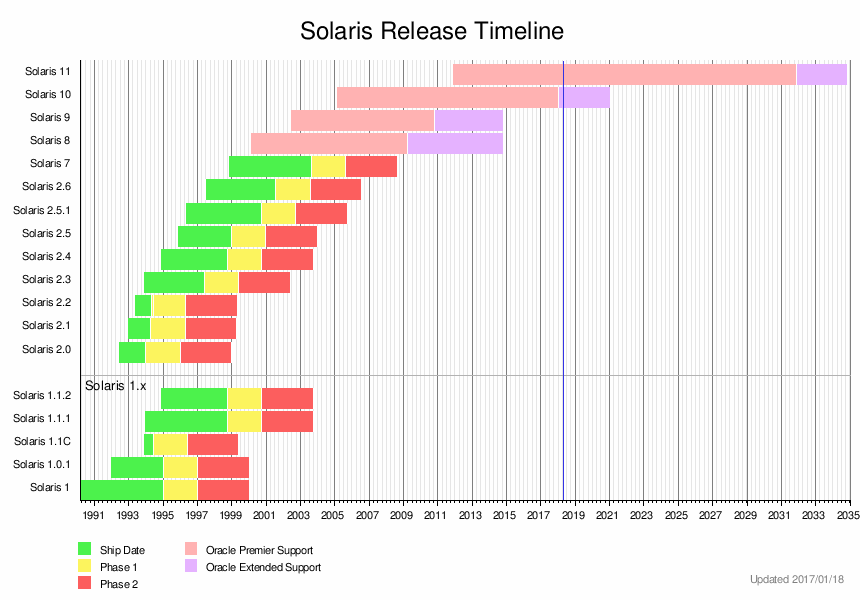
\includegraphics[scale=0.5]{img/releases.png}
\caption{Sistema de Archivos Disponible}
\label{fig:dis2}
\end{figure}
\end{center}

El 9 de noviembre de 2011 Oracle (ya adquirida Sun) presentó Solaris 11, la última versión disponible esta cerro el desarrollo comercial de Solaris debido a problemas de marketing y posicion de mercado. 
Solaris tiene las siguientes caracteristicas 
\begin{enumerate}
\item PORTABILIDAD: El software conformado por una ABI aplicación de interfaces binaria (Application Binary Interface) ejecuta con un Shrink-wrapped (Contracción envuelta) el software en todos los sistemas vendidos con la misma arquitectura del microprocesador. Esto obliga a los desarrolladores de aplicaciones a reducir el costo del desarrollo del software y traer productos al mercado rápidamente, y obliga a los usuarios a actualizar el hardware mientras retienen sus aplicaciones de software y minimizan sus costos de conversión.
\item ESCALABILIDAD: Las aplicaciones se usan con más frecuencia en el sobre tiempo, y requiere sistemas más poderosos para soportarlos. Para operar en un ambiente creciente, el software debe ser capaz de ejecutar en un rango de ancho poderosos y debe ser capaz de tomar ventajas del poder adicional que se está procesando.
\item INTEROPERATIBIDAD: La computación del ambiente heterogéneo es una realidad hoy. Los usuarios compran de muchos vendedores para implementar la solución que necesitan. La estandarización y una clara interface son criterios para un ambiente heterogéneo, permitiendo a los usuarios desarrollar estrategias para comunicarse por medio de su red. El sistema operativo de Solaris puede interoperar con unos sistemas muy populares hoy en el mercado, y aplicaciones que se ejecutan en UNIX se pueden comunicar fácilmente.
\item COMPATIBILIDAD: La tecnología de la computación continua avanzando rápidamente, pero necesita permanecer en el ámbito competitivo para minimizar sus costos y maximizar sus ingresos.
\end{enumerate}

\section{Proceso de instalación Unix System V R4}
\begin{figure}[H]
 	\centering
   	\subfloat[Bienvenida Instalador Unix System V R4]{\label{fig:bienvenida}{
   		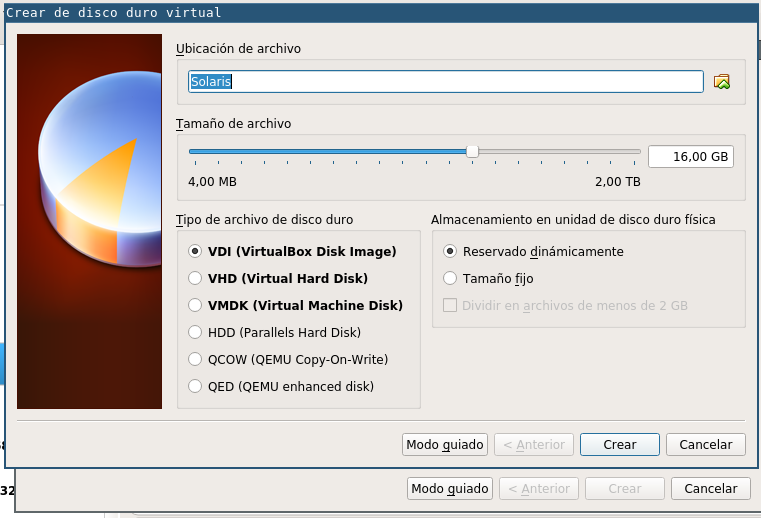
\includegraphics[width=0.68\textwidth]{img/2.png}
   		}}
	\subfloat[Aceptando terminos de instalacion de Unix]{\label{fig:formateada}{
   		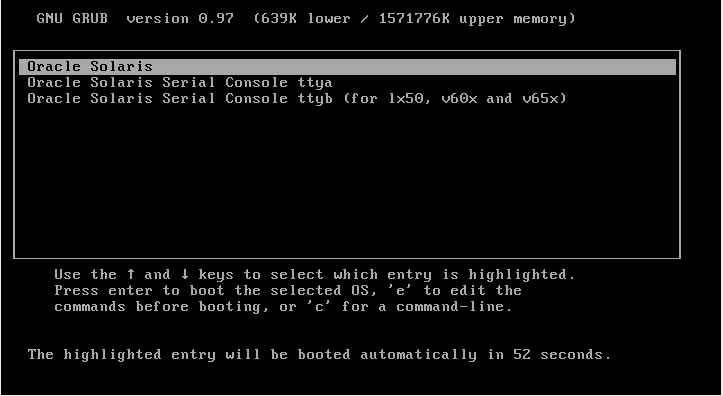
\includegraphics[width=0.68\textwidth]{img/3.png}
        }}
       \hfill
	\subfloat[Utilizaremos 100\% del disco  para la instalacion.]{\label{fig:disco}{
   		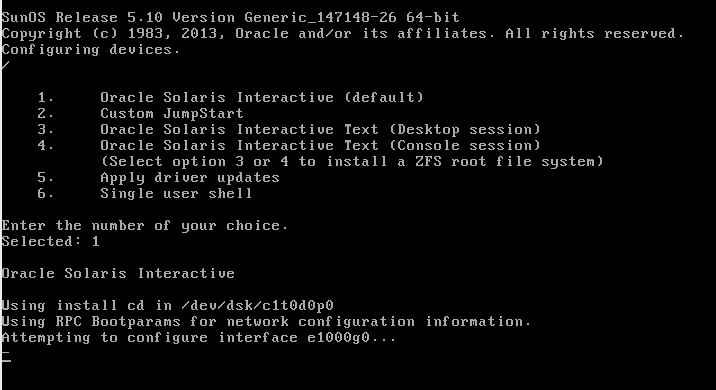
\includegraphics[width=0.68\textwidth]{img/4.png}
        }}
	\subfloat[Seleccion  del Sistema de Archivos para la Instalacion\textit{ufs}]{\label{fig:ufs}{
   		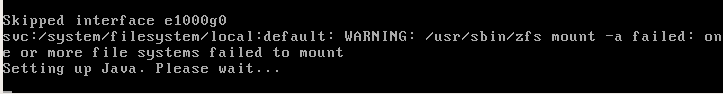
\includegraphics[width=0.68\textwidth]{img/5.png}
        }}
        \hfill
	\subfloat[Confirmación de particiones y ubicación de instalación.]{\label{fig:confirmar}{
   		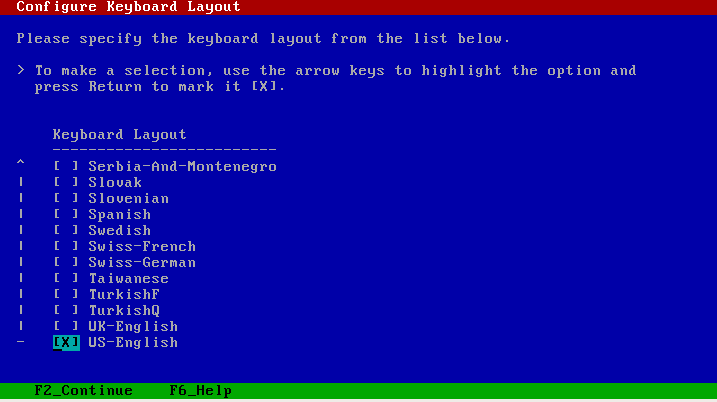
\includegraphics[width=0.68\textwidth]{img/6.png}
        }}
	\subfloat[El sistema decide los tamaños para las particiones.]{\label{fig:particiones}{
   		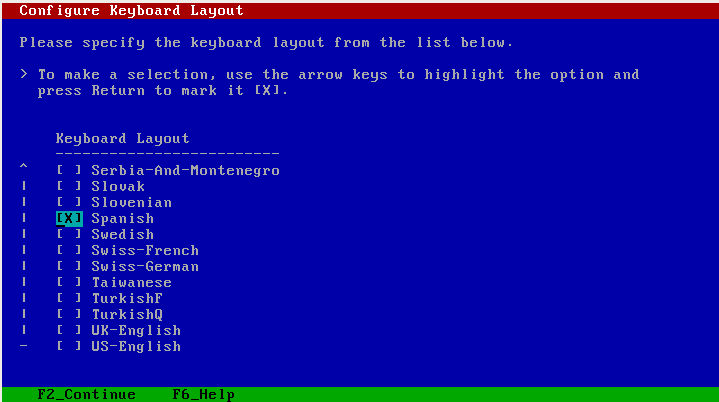
\includegraphics[width=0.68\textwidth]{img/7.png}
        }}
	\caption{Configuración inicial de instalación}
\end{figure}

\begin{figure}[H]
 	\centering
   	\subfloat[]{\label{fig:bienvenida}{
   		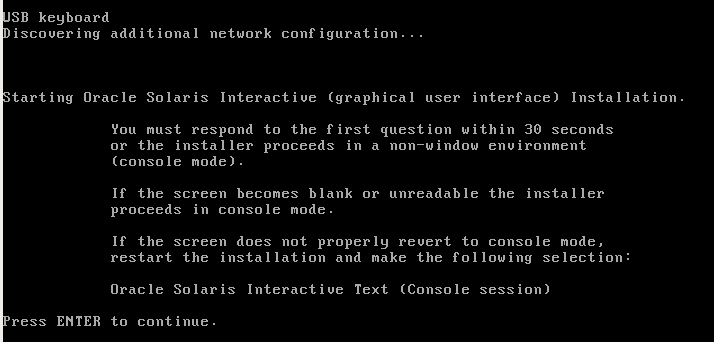
\includegraphics[width=0.68\textwidth]{img/8.png}
   		}}
	\subfloat[]{\label{fig:formateada}{
   		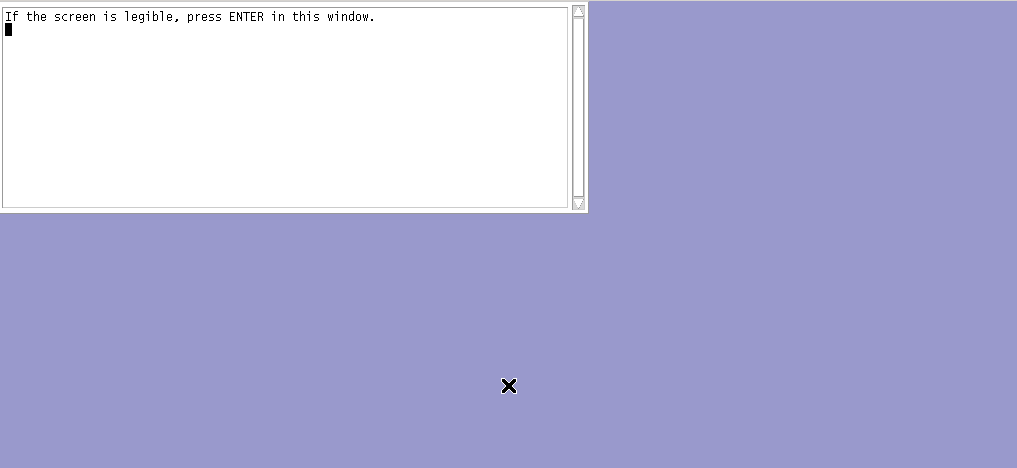
\includegraphics[width=0.68\textwidth]{img/9.png}
        }}
       \hfill
	\subfloat[]{\label{fig:disco}{
   		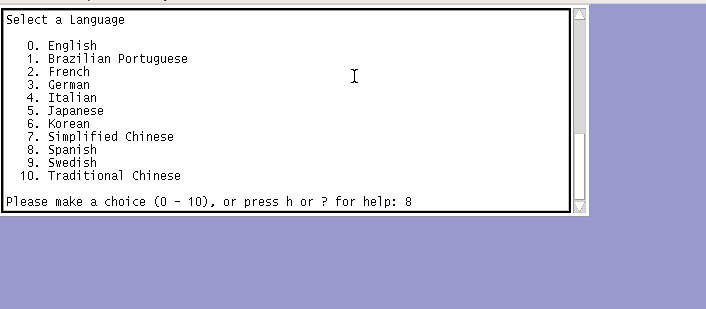
\includegraphics[width=0.68\textwidth]{img/10.png}
        }}
      \subfloat[Ultimo Diskette 10 de 10]{\label{fig:ufs}{
   		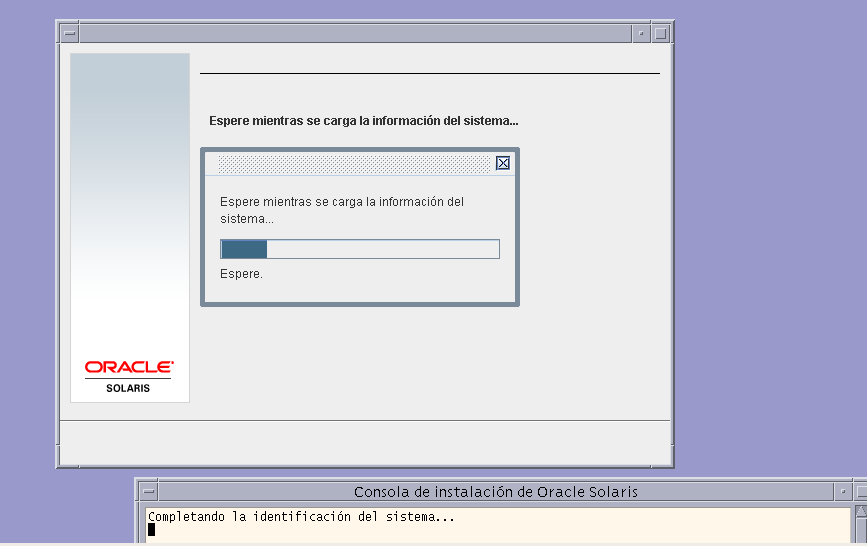
\includegraphics[width=0.68\textwidth]{img/11.png}
        }}
	\caption{Proceso secuencial de instalación, intercambio de diskettes}
\end{figure}

\section{Manejo de Archivos y Estructura}
El manejo de archivos en Solaris en su version 10 se puede realizar mediante  el administrador de archivos y ventanas que trae por defecto el, tambien como se describe en los \fnurl{oficiales}{https://docs.oracle.com/cd/E19455-01/806-1360/6jalch31j/index.html} El manejo de archivos en Solaris te permite :
\begin{itemize}
\item Manipular y administrar carpetas 
\item Navegación sencilla sobre el sistema de archivos
\item Administrar permisos de los archivos 
\item Realizar búsquedas rápidas sobre el sistema de archivos
\item Personalizar vista del sistema de archivos
\item Administrar dispositivos de almacenamiento externos
\end{itemize}
%Formato imagen unica
\section{Clasificación del Sistema Operativo}
Este sistema operativo se clasifica como : 
\begin{itemize}
\item Multiproceso 
\item Multiusuario
\item Multitarea
\item Proppósito general
\item Micronúcleo
\item Abierto
\end{itemize}

\section{Ejecucion Comandos}
Para realizar la ejecución de comandos en el sistema operativo Solaris nos valemos de la ayuda provista por el \fnurl{profesor}{http://sparcki.blogspot.com.co/2009/09/comandos-basicos-y-no-tan-basicos-de.html}

En esta ayuda hay mas de 20 comandos que nos permiten ver algunas cosas interesantes, para ello utilizaremos la shell que nos provee el sistema operativo instalado. 

\begin{figure}[H]
 	\centering
   	\subfloat[Identificación de version,  usuario que ejecuta los comandos y obtencion de identificacion.]{\label{fig:cmd1}{
   		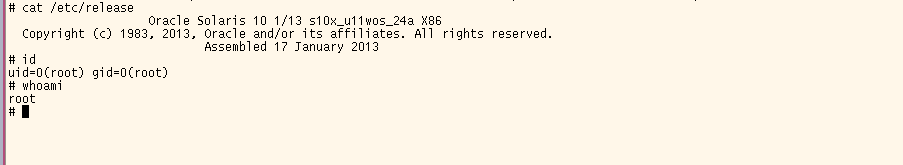
\includegraphics[width=0.68\textwidth]{img/c1.png}
   		}}
	\subfloat[cambiar el planificador por defecto en Solaris,ayuda del planificador]{\label{fig:cmd2}{
   		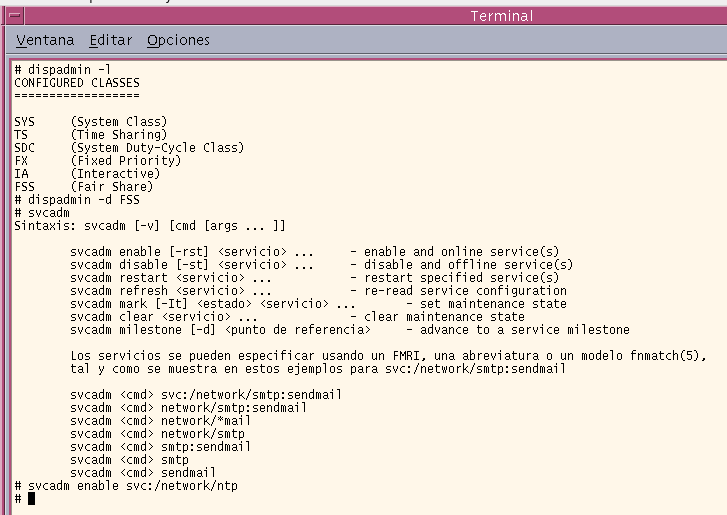
\includegraphics[width=0.68\textwidth]{img/c2.png}
        }}
       \hfill
	\subfloat[Conocer detalles de CPU instaladas y reconocidas OpenSolaris.]{\label{fig:cmd3}{
   		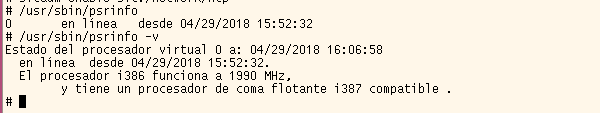
\includegraphics[width=0.68\textwidth]{img/c3.png}
        }}
	\subfloat[Obtener detalles de Procesos con ps, múltiples comandos de ps.]{\label{fig:cmd4}{
   		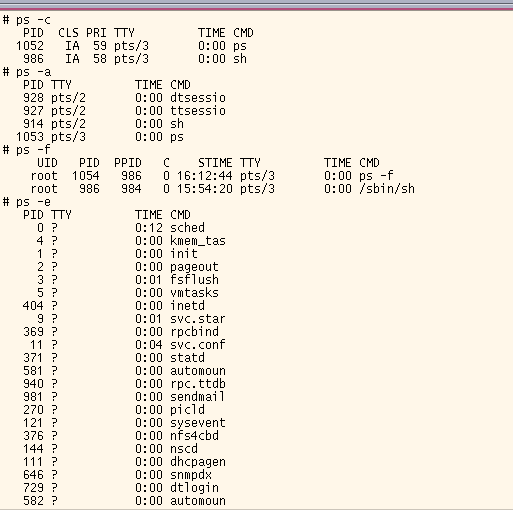
\includegraphics[width=0.68\textwidth]{img/c4.png}
        }}
        \hfill
	\subfloat[Obtener la lista de recursos asociados a un procesos.]{\label{fig:cmd5}{
   		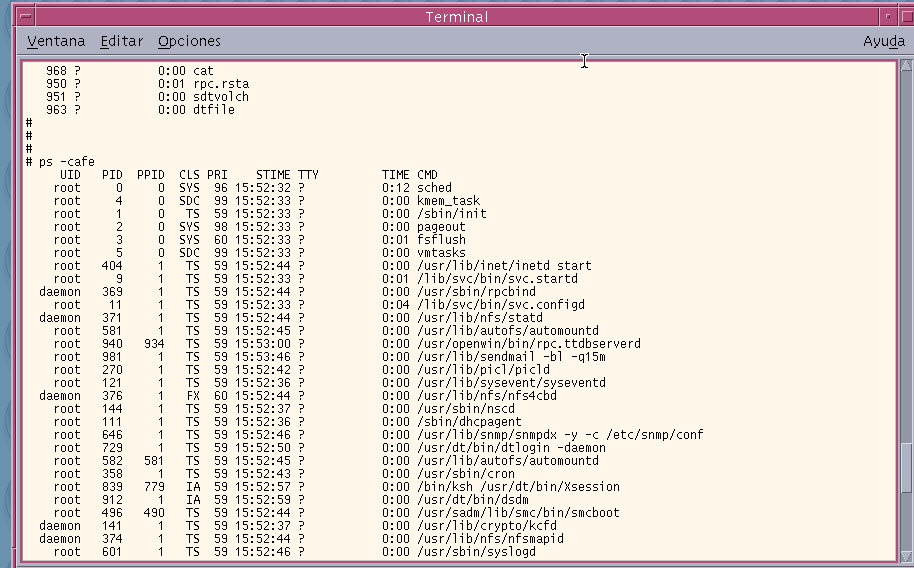
\includegraphics[width=0.68\textwidth]{img/c5.png}
        }}
	\subfloat[Conocer Dispositivos de hardware, arquitectura soportada. Conocer el project de usuario.]{\label{fig:particiones}{
   		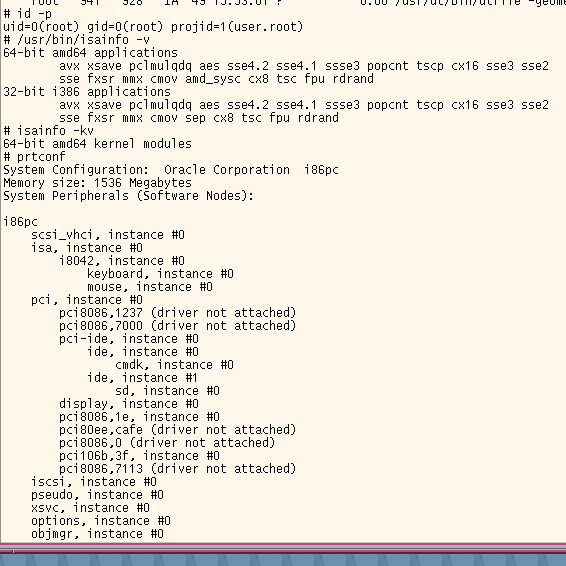
\includegraphics[width=0.68\textwidth]{img/c6.png}
        }}
	\caption{Listado de Comandos Múltiples}
\end{figure}

\begin{figure}[H]
 	\centering
   	\subfloat[Identificar ultimo inicio del sistema operativo, fecha del sistema operativo, y variables de entorno de un pid]{\label{fig:cmd7}{
   		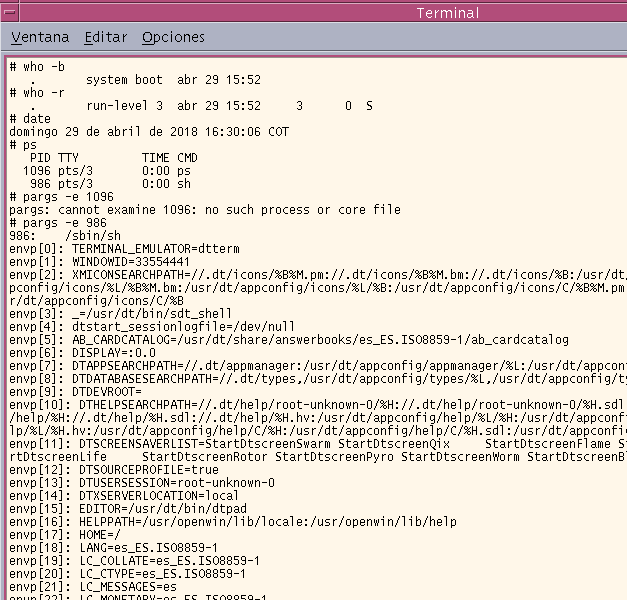
\includegraphics[width=0.68\textwidth]{img/c7.png}
   		}}
	\subfloat[Verificacion de Conexión con sitios a internet, firefox desde terminal, y uso de ping.]{\label{fig:cmd8}{
   		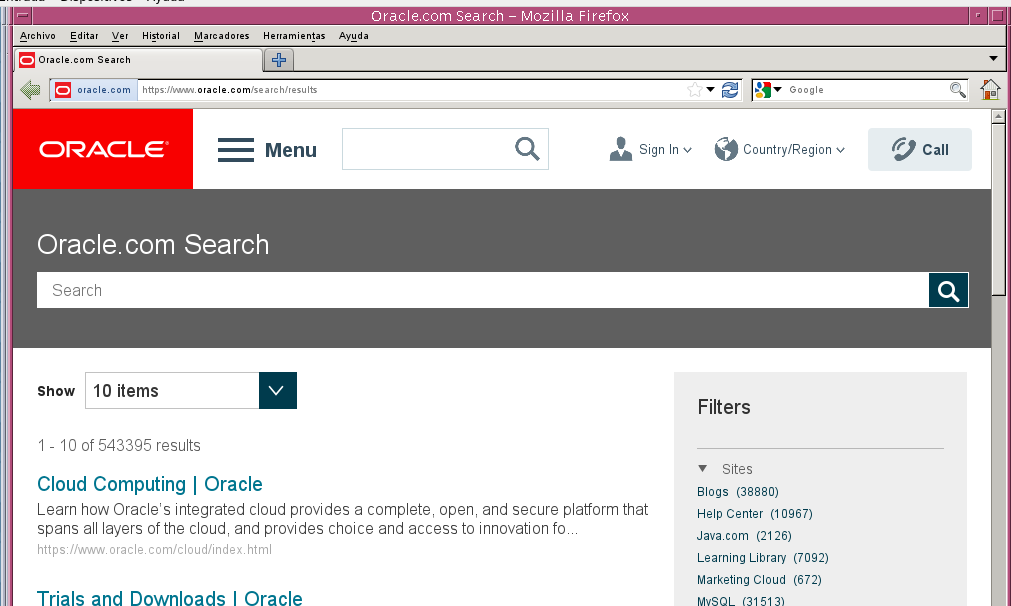
\includegraphics[width=0.68\textwidth]{img/c8.png}
        }}
       \hfill
	\subfloat[Verificacion de conexión]{\label{fig:cmd3}{
   		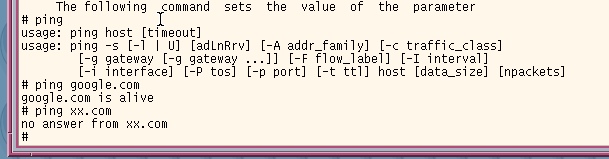
\includegraphics[width=0.68\textwidth]{img/c71.png}
        }}
	\subfloat[Habilitar IPV4 Forwarding y verificar estado]{\label{fig:cmd9}{
   		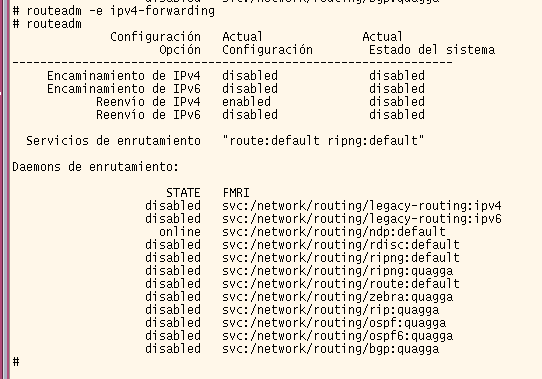
\includegraphics[width=0.68\textwidth]{img/c9.png}
        }}
        \hfill
	\subfloat[Herramientas de Test de Solaris - AMT Common Criteria Security]{\label{fig:cmd10}{
   		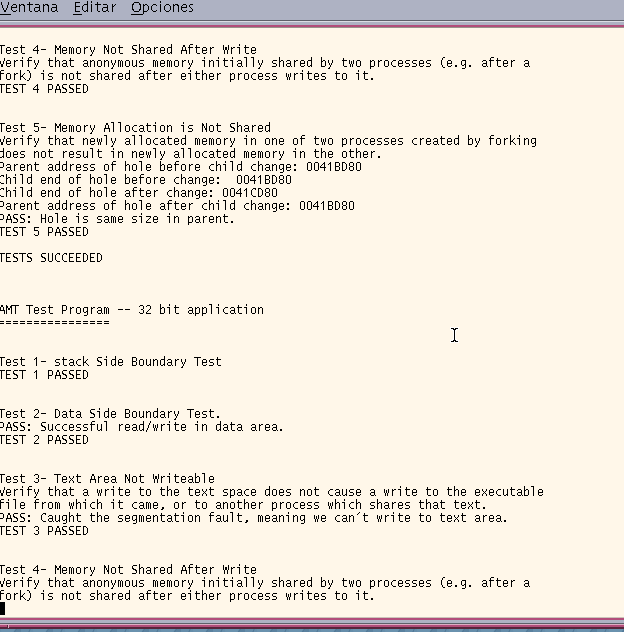
\includegraphics[width=0.68\textwidth]{img/c10.png}
        }}
	\subfloat[Conocer Dispositivos de hardware, arquitectura soportada. Conocer el project de usuario.]{\label{fig:particiones}{
   		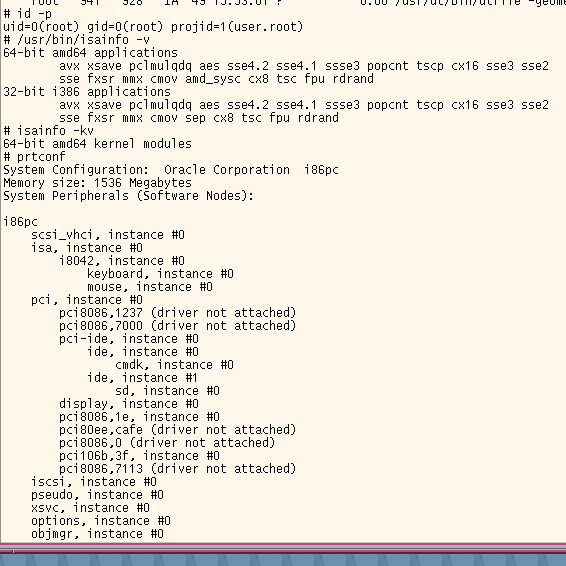
\includegraphics[width=0.68\textwidth]{img/c6.png}
        }}
	\caption{Configuración inicial de instalación}
\end{figure}
\section{Referencias}
\begin{itemize}
\item  \hyperref[http://sparcki.blogspot.com.co/2009/09/comandos-basicos-y-no-tan-basicos-de.html]{Todo Sobre Solaris Sparcki blog}
\end{itemize}
\end{document}